\documentclass[a4paper,10pt]{article}
\usepackage[utf8]{inputenc}
\usepackage{graphicx}
\usepackage{framed} 
\usepackage{xcolor}
\usepackage{tcolorbox}
\usepackage{xcolor} 
\colorlet{shadecolor}{gray!25}
\definecolor{mshadecolor}{rgb}{0.7421875,0.7421875,0.7421875}

%opening
\title{Offensive Security\\
	Lab-report
}
\author{Moritz Rupp}
\begin{document}

\maketitle
\tableofcontents
\begin{abstract}
Lab3 documentation
\end{abstract}
\newpage
\section{Exercise 3}
\subsection{UART Communication Analysis}
Salea offers an extension 'Saleae-Hex-Ascii-Dec-to-Terminal` that is capable of converting low level analyser output to human readable data. This way we can write the bewished encoding like ascii to a file of choice.\\
With the help of a simple Python script, it's now possible to read out the flag.
\begin{center}
 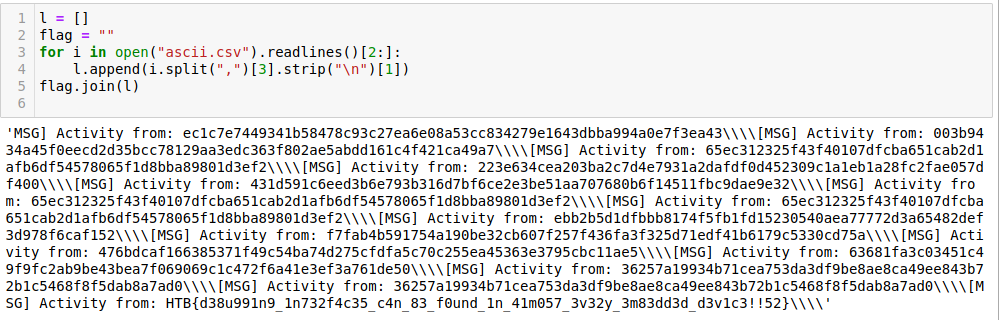
\includegraphics[scale=0.4]{3.1.png}
\end{center}
\subsection{Binary Data Analaysis}
Using the shell commands 'file' we discover that the provided image is an 'Linux kernel ARM boot executable zImage'. After some research we are able to extract all contents of the Image.
\begin{center}
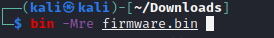
\includegraphics[scale=0.6]{binwalk.png}
\end{center}
This results in a folder '\_firmware.bin.extracted\/' that contains a full linux file system. At first i tought we could find the flag within one of the files and folders, but didnt succeed.
So the next step was to scan the host via nmap. We discover that the machine is running a telnet busy box. So naturally i try to connect to the host ip via telnet which prompts me to enter credentials. After failing with standart logins such as 'admin:admin' etc.,  I search the file system for telnet credentials. Via grep im able to find an interesting file 'telnet.sh'.
\begin{center}
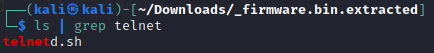
\includegraphics[scale=0.5]{telnet.png}
\end{center}
In there we can find the username 'Device\_Admin' and a hint for the password, which lays in the file 'sign' that can be found within the file system.
\begin{center}
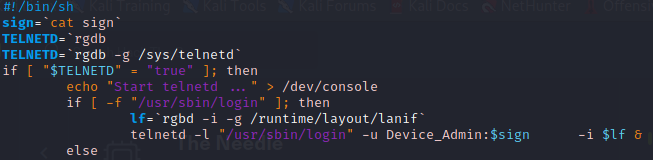
\includegraphics[scale=0.5]{telnetf.png} 
\end{center}
\newpage
After connecting to the telnet service, we find the flag there.
\begin{center}
 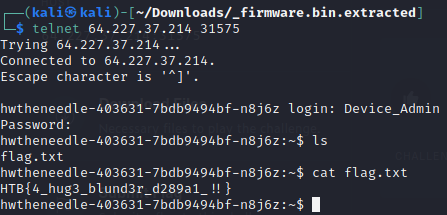
\includegraphics[scale=0.5]{flag.png}
\end{center}
\subsection{Password Cracking - Timing Side Channel Attack}
At first we try to guess the length of the password.
We achive this by calling the function 'password\_check()' with increasing amounts of input length(line 7).
When we measure the time before and after the function call(line 6,8) we can tell how long the computation took. Due to the design of the function, correct inputs will take longer to compute, hence we look for the hightest nummber of computation times.
\begin{center}
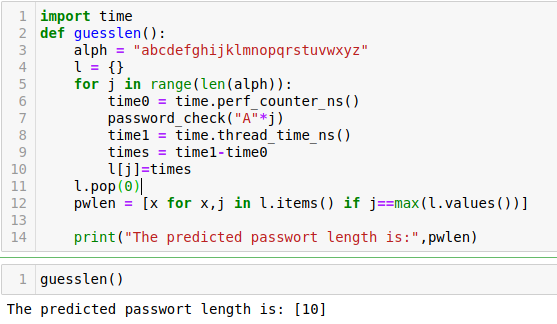
\includegraphics[scale=0.5]{guesslen.png} 
\end{center}
In line 10 we write the input length as a key with the corresponding value to a dict. Since the first 'round' is always the longest, we get rid of it in line 11.
The list comprehension in line 12 extracts the key of the biggest value which represents the predicted length. The correct guess is 10!\\
The next task is to find the correct password characters. We can achieve this by applying the same method.\\
\newpage
\noindent At first we have to generate the payload for testing. Since we know that the passwort length is 10 chars, we create a list with 10 empthy strings. We fill those strings with different starting chars and input them in the function. 
\begin{center}
 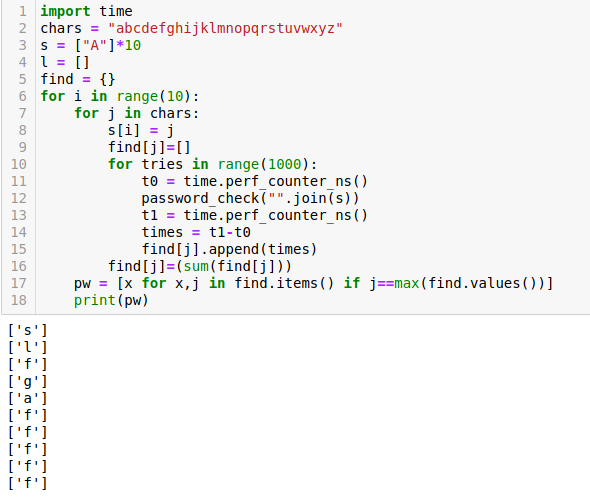
\includegraphics[scale=0.5]{pw.png}
\end{center}
Using the same method like in our previous function, we can now try to find the right char! But since python in Jupyter Notebook is awfully inconsistent and runs like garbage we're failing to guess the correct passwort characters.
\subsection{Password Cracking - Simple Power Analysis Attack}
\end{document}
